%% ----------------------------------------------------------------
%%? 1st Draft In Progress (2 days left)
%%* 10,400/10K words
%% ----------------------------------------------------------------
\documentclass{src/ecsgdp}
\graphicspath{ {./images/} }
\hypersetup{colorlinks=true}
%% ----------------------------------------------------------------
%% Definitions.tex
%% ---------------------------------------------------------------- 
\newcommand{\BibTeX}{{\rm B\kern-.05em{\sc i\kern-.025em b}\kern-.08em T\kern-.1667em\lower.7ex\hbox{E}\kern-.125emX}}

%% People
\newcounter{address}
\setcounter{address}{1}
\renewcommand{\theaddress}{\textsuperscript{\fnsymbol{address}}}
\newcommand{\address}[1]{\refstepcounter{address}\theaddress#1\\}
\newcommand{\Name}[3]{\texorpdfstring{\href{mailto:#3}{#2}#1}{#2}\xspace}

%% Dingbats
\newcommand{\tick}{\ding{51}}
\newcommand{\cross}{\ding{55}}

%% Calculus
\newcommand{\pd}[2]{\ensuremath{\frac{\partial #1}{\partial #2}}\xspace}
\newcommand{\fd}[2]{\ensuremath{\frac{d #1}{d #2}}\xspace}
\newcommand{\dint}{\ensuremath{\int\!\!\!\int}\xspace}
\newcommand{\tint}{\ensuremath{\int\!\!\!\int\!\!\!\int}\xspace}

%% Math Sets
\newcommand{\Q}[1]{\ensuremath{\mathbb{#1}}\xspace}
\newcommand{\R}{\Q{R}}

%% Matrix, Vector
\newcommand{\V}[1]{\ensuremath{\boldsymbol{#1}}\xspace}
\newcommand{\M}[1]{\ensuremath{\boldsymbol{#1}}\xspace}
\newcommand{\0}{\V{0}}
\newcommand{\1}{\V{1}}
\newcommand{\I}{\M{I}}

%% Math Functions
\newcommand{\F}[1]{\ensuremath{\mathrm{#1}}\xspace}
\newcommand{\sgn}{\F{sgn}}
\newcommand{\tr}{\F{trace}}
\newcommand{\diag}{\F{diag}}

%% Math Names
\newcommand{\N}[1]{\ensuremath{\mathit{#1}}\xspace}

%% Data
\newcommand{\mc}[1]{\ensuremath{\mathcal{#1}}\xspace}
\newcommand{\Hyp}{\mc{H}}
\newcommand{\D}{\mc{D}}

%% Kernel
\newcommand{\K}{\M{K}}
\newcommand{\eins}{\texorpdfstring{\ensuremath{\epsilon}}{\textepsilon}-insensitive\xspace}
\newcommand{\e}{\ensuremath{\epsilon}\xspace}
\newcommand{\Bxi}{\ensuremath{\boldsymbol{\xi}}\xspace}
\newcommand{\Kanova}{\ensuremath{\mathit{K_{ANOVA}}}\xspace}
\newcommand{\Kspline}{\ensuremath{\mathit{K_{spline}}}\xspace}

%% Bayesian
\newcommand{\MP}{\ensuremath{\mathit{{\scriptscriptstyle \hspace{-1.5pt}M\hspace{-1.5pt}P}}}\xspace}
\newcommand{\ML}{\ensuremath{\mathit{{\scriptscriptstyle \hspace{-1.5pt}M\hspace{-1.5pt}L}}}\xspace}
\newcommand{\Qw}{\ensuremath{Q_{\w}(\w)}\xspace}
\newcommand{\Qa}{\ensuremath{Q_{\Ba}(\Ba)}\xspace}
\newcommand{\Qb}{\ensuremath{Q_{\beta}(\beta)}\xspace}
\newcommand{\wMPab}{\ensuremath{\w_{\MP|\bar {\Ba},\bar \beta}}\xspace}
\newcommand{\wMP}{\ensuremath{\w_{\MP}}\xspace}
\newcommand{\yMP}{\ensuremath{y_{\MP}}\xspace}
\newcommand{\BaMP}{\ensuremath{\Ba_{\hspace{1pt}\MP}}\xspace}
\newcommand{\aMP}{\ensuremath{\alpha_{\hspace{1pt}\MP}}\xspace}
\newcommand{\bMP}{\ensuremath{\beta_{\hspace{1pt}\MP}}\xspace}
\newcommand{\Sab}{\ensuremath{\M{\Sigma}_{\bar \Ba,\bar \beta}}\xspace}
\newcommand{\Ba}{\ensuremath{\boldsymbol{\alpha}}\xspace}
\newcommand{\Bb}{\ensuremath{\boldsymbol{\beta}}\xspace}
\newcommand{\Bm}{\ensuremath{\boldsymbol{\mu}}\xspace}
\newcommand{\BL}{\ensuremath{\boldsymbol{\Lambda}}\xspace}
\newcommand{\BPhi}{\ensuremath{\boldsymbol{\Phi}}\xspace}
\newcommand{\SMP}{\ensuremath{\M{\Sigma}_{\MP}}\xspace}

\newcommand{\Pa}{\ensuremath{P(\alpha|\mathcal{H})}\xspace}
\newcommand{\Pb}{\ensuremath{P(\beta|\mathcal{H})}\xspace}
\newcommand{\Pab}{\ensuremath{P(\alpha,\beta|\mathcal{H})}\xspace}
\newcommand{\Pw}{\ensuremath{P(\w|\mathcal{H})}\xspace}
\newcommand{\PD}{\ensuremath{P(\D|\mathcal{H})}\xspace}
\newcommand{\PwIa}{\ensuremath{P(\w|\alpha,\mathcal{H})}\xspace}
\newcommand{\PDIwb}{\ensuremath{P(\D|\w,\beta,\mathcal{H})}\xspace}
\newcommand{\PDwab}{\ensuremath{P(\D,\w,\alpha,\beta|\mathcal{H})}\xspace}
\newcommand{\PDIw}{\ensuremath{P(\D|\w,\mathcal{H})}\xspace}
\newcommand{\PwID}{\ensuremath{P(\w|\D,\mathcal{H})}\xspace}
\newcommand{\PwabID}{\ensuremath{P(\w,\alpha,\beta|\D,\mathcal{H})}\xspace}

\newcommand{\PanH}{\ensuremath{P(\alpha)}\xspace}
\newcommand{\PbnH}{\ensuremath{P(\beta)}\xspace}
\newcommand{\PabnH}{\ensuremath{P(\alpha,\beta)}\xspace}
\newcommand{\PwnH}{\ensuremath{P(\w)}\xspace}
\newcommand{\PDnH}{\ensuremath{P(\D)}\xspace}
\newcommand{\PwIanH}{\ensuremath{P(\w|\alpha)}\xspace}
\newcommand{\PDIwbnH}{\ensuremath{P(\D|\w,\beta)}\xspace}
\newcommand{\PDwabnH}{\ensuremath{P(\D,\w,\Ba,\beta)}\xspace}
\newcommand{\PDIwnH}{\ensuremath{P(\D|\w)}\xspace}
\newcommand{\PwIDnH}{\ensuremath{P(\w|\D)}\xspace}
\newcommand{\PwabIDnH}{\ensuremath{P(\w,\alpha,\beta|\D)}\xspace}

\newcommand{\PDwBab}{\ensuremath{P(\D,\w,\Ba,\beta|\mathcal{H})}\xspace}
\newcommand{\PwIBa}{\ensuremath{P(\w|\Ba,\mathcal{H})}\xspace}
\newcommand{\PBab}{\ensuremath{P(\Ba,\beta|\mathcal{H})}\xspace}
\newcommand{\PwBabID}{\ensuremath{P(\w,\Ba,\beta|\D,\mathcal{H})}\xspace}

\newcommand{\PBanH}{\ensuremath{P(\Ba)}\xspace}
\newcommand{\PwIBanH}{\ensuremath{P(\w|\Ba)}\xspace}

%% Snakes
\newcommand{\Esnake}{\ensuremath{\mathit{E_{snake}}}\xspace}
\newcommand{\Eimage}{\ensuremath{\mathit{E_{image}}}\xspace}
\newcommand{\Econt}{\ensuremath{\mathit{E_{cont}}}\xspace}
\newcommand{\Ecurv}{\ensuremath{\mathit{E_{curv}}}\xspace}
\newcommand{\Eint}{\ensuremath{\mathit{E_{int}}}\xspace}
\newcommand{\Eext}{\ensuremath{\mathit{E_{ext}}}\xspace}
\newcommand{\Eterm}{\ensuremath{\mathit{E_{term}}}\xspace}
\newcommand{\Eline}{\ensuremath{\mathit{E_{line}}}\xspace}
\newcommand{\Eedge}{\ensuremath{\mathit{E_{edge}}}\xspace}
\newcommand{\Econ}{\ensuremath{\mathit{E_{con}}}\xspace}
\newcommand{\Eangle}{\ensuremath{\mathit{E_{angle}}}\xspace}
\newcommand{\Elshape}{\ensuremath{\mathit{E_{lshape}}}\xspace}
\newcommand{\Eedgedir}{\ensuremath{\mathit{E_{edgedir}}}\xspace}
\newcommand{\Emodel}{\ensuremath{\mathit{E_{model}}}\xspace}
\newcommand{\wte}{\ensuremath{\mathit{w_{term}}}\xspace}
\newcommand{\wli}{\ensuremath{\mathit{w_{line}}}\xspace}
\newcommand{\wed}{\ensuremath{\mathit{w_{edge}}}\xspace}
\newcommand{\wco}{\ensuremath{\mathit{w_{con}}}\xspace}

%% Environments
\newcounter{alg}
\newenvironment{algorithm}[1]
{
    \stepcounter{alg}
    \begin{table}[htb]
    \centering
    \begin{tabular}[t]{ll}
    \hline&\\
    \multicolumn{2}{l}{\bf Algorithm \arabic{alg}: #1}\\&\\
} {
    &\\
    \hline
    \end{tabular}
    \end{table}
}


\usepackage{multirow}
\usepackage{longtable}

%% ----------------------------------------------------------------
\begin{document}
\frontmatter
\title{Project Audyssey - A Platform for Multidimensional Journeys through Large Song Libraries}
\authors    {{Kathirvelan Arounassalam}}
\date       {April 10, 2025}
% \keywords   {}
\supervisor {David Millard}
\examiner   {Zehor Belkhatir}
%\
\degree     {Bachelor's in Computer Science}
\reporttype {project report} % Change here if you're doing a 3YP report
\maketitle

\begin{abstract}
%% ----------------------------------------------------------------
%% Max 200 words
%% ----------------------------------------------------------------
\end{abstract}

\textbf{Statement of Originality}
\begin{itemize}
    \item I have read and understood the ECS Academic Integrity information and the University’s Academic Integrity Guidance for Students.
    \item I am aware that failure to act in accordance with the Regulations Governing Academic Integrity may lead to the imposition of penalties which, for the most serious cases, may include termination of programme.
    \item I consent to the University copying and distributing any or all of my work in any form and using third parties (who may be based outside the EU/EEA) to verify whether my work contains plagiarised material, and for quality assurance purposes.
\end{itemize}

We expect you to acknowledge all sources of information (e.g. ideas, algorithms, data) using citations. You must also put quotation marks around any sections of text that you have copied without paraphrasing. If any figures or tables have been taken or modified from another source, you must explain this in the caption and cite the original source.

\textbf{I have acknowledged all sources, and identified any content taken from elsewhere.}

If you have used any code (e.g. open-source code), reference designs, or similar resources that have been produced by anyone else, you must list them in the box below. In the report, you must explain what was used and how it relates to the work you have done.

The JavaScript React library \href{https://www.ag-grid.com/react-data-grid/getting-started/}{\texttt{ag-grid-react}} was used to implement the table fiew for the application.

\textbf{I have not used any resources produced by anyone else.}

You can consult with module teaching staff/demonstrators, but you should not show anyone else your work (this includes uploading your work to publicly-accessible repositories e.g. Github, unless expressly permitted by the module leader), or help them to do theirs. For individual assignments, we expect you to work on your own. For group assignments, we expect that you work only with your allocated group. You must get permission in writing from the module teaching staff before you seek outside assistance, e.g. a proofreading service, and declare it here.

\textbf{I did all the work myself, or with my allocated group, and have not helped anyone else.}

We expect that you have not fabricated, modified or distorted any data, evidence, references, experimental results, or other material used or presented in the report. You must clearly describe your experiments and how the results were obtained, and include all data, source code and/or designs (either in the report, or submitted as a separate file) so that your results could be reproduced.

\textbf{The material in the report is genuine, and I have included all my data/code/designs.}

We expect that you have not previously submitted any part of this work for another assessment. You must get permission in writing from the module teaching staff before re-using any of your previously submitted work for this assessment.

\textbf{I have not submitted any part of this work for another assessment.}

If your work involved research/studies (including surveys) on human participants, their cells or data, or on animals, you must have been granted ethical approval before the work was carried out, and any experiments must have followed these requirements. You must give details of this in the report, and list the ethical approval reference number(s) in the box below.

\textbf{My work did not involve human participants, their cells or data, or animals.}


\tableofcontents
\listoffigures
\listoftables
\lstlistoflistings

%% ----------------------------------------------------------------
% Optional extra pages
%\listofsymbols{ll}{$w$ & The weight vector}
%\acknowledgements{Here are some acknowledgements}
%\dedicatory{To \dots}
%% ----------------------------------------------------------------

% \mainmatter means that we've gone from i, ii, iii, iv, v etc.
% introduction numbering to 1,2,3,4,5 chapter numbering

\mainmatter

% -------------------------------------------------
% Introduction to the Problem
% -------------------------------------------------
%% ----------------------------------------------------------------
%%? (1st Draft Complete)
%% ----------------------------------------------------------------
\chapter{Introduction (870 words)}% \label{Chapter:Introduction}
%This template was originally from \cite{Gunn:2001:pdflatex}.
\section{Problem}
As technology has advanced over the years, people's personal music collections have become more and more digital \cite{
    %cite the streaming percentage
}.

Initially, if a listener wanted to listen to a song or some music, it would have to be performed live, usually by the creator of said music. As such music started to be performed in concerts, where many people could listen to songs from one or more artists.

Radio allowed people to listen to music together and in the comfort of their own home. However, there wasn't full control over what to listen to.

Vinyls and CDs allowed for listening to any song in any place, with the right equipment. This made it possible for people to start treating music as a collectible physical item and build personal music collections. However these physical collections were limited by purchase cost and storage space.

As technology progressed further, we entered the streaming era, where physical collections were replaced by digital collections. These digital collections are significantly cheaper, and are much less constrained by storage space.

As such music collections have the capability to be significantly larger than their physical counterpart. The process of adding songs is much simpler digitally, allowing these digital collections to grow at a significantly faster rate than physical collections.

To navigate the landscape of a personal music collection the predominant method employed by streaming applications is to simply arrange the items in a list. This method works well on a small scale, but falls apart with the large scale that digital music collections can reach.

As such, as a workaround, most users split their mental collections into sub-collections (playlist)s, folders that allow for a lesser mental load and better maintainability.

Whilst playlists help manage the scale of songs, they themselves' have the issue "when a user’s playlists become overwhelmingly numerous, streaming services begin to appear inefficient and unmanageable as collection systems"\cite{playlistExperience}.

This hierarchical system allows for the better handling of large scale collections that grow at the pace most collections do \textbf{CITE} but if these playlists grow too large, then they require reorganising which can become a chore.

As such the organisational benefit provided by these playlists is lost due to the 'perceived' high mental load required.

Whilst the capability and format of personal music collections have changed dramatically with technological advancements, the structure of these collections has stagnated in the streaming era.

This project will investigate different structures to see how they can improve either of the following key aspects for personal music collections:\begin{itemize}
    \item \textbf{
        Complete Knowledge of the Collection
    } - understanding the entire contents of the collection (to not lose/forget about songs in the collection over time) without exacting a heavy mental load
    \item \textbf{
        Replayability/Queue Building
    } - being able to quickly and frictionlessly create song queues to listen to (where the order of the song queue exists on a spectrum between fixed and random)
\end{itemize}
%! How do I show that these have stagnated

\section{Method}
First we will try to understand people's mental organisational models for their personal music collections and how they create song queues using their organisational model.

Then we will see the relationship between their mental understanding and their digital music collection.

\subsection{Complete Knowledge over the Collection}
For song organisation, the current method employed by streaming applications is a folder-based list structure (using playlists as folders).

Other methods using graphical spatial methods have been researched\begin{itemize}
    \item there has been research into creating 2d and 3d visualisations of song Libraries
    \item although there hasn't been research into making these usable from a software application point of view
\end{itemize}

%todo do I need to give examples or find way to better explain this
This project will employ three different organisational models:\begin{itemize}
    \item \textbf{Clustered Table} \(\to\) %! Do I keep this here?
    \item \textbf{Static Graph} \(\to\) each song is mapped onto a cartesian grid (both 2D and 3D) where the co-ordinates of the song is determined by the numerical attribute for that axis
    \item \textbf{Dynamic Graph} \(\to\) each song is spaced out from every other song depending on how similar they are to each other, based on both metadata (artist, genre, etc.) and attributes
\end{itemize}

The aforementioned attributes are mid-level features analysed from the audiofile of each song \(\to\) these include the instrumentalness, loudness, energy, etc. of a track
% these attributes will be pulled from Spotify's API as that works well if I look at people with Spotify Libraries

\subsection{Replayability/Queue Building}
When listening to songs, the next song to be played is chosen somewhere on a spectrum between fully deterministically (manually selected) or fully non-determinstically (randomly selected):\begin{itemize}
    \item fixed deterministic choices occur when the listener knows which song they want to listen to next
    \item when the listener doesn't know which song to listen to next then the next song should be randomly chosen (such as with Spotify's shuffle feature on a playlist)
\end{itemize}

With the advent of software now being the medium with which songs are listened to, song queues can now be generated randomly from a set of songs, such as a listener's playlist.

However, there exists no framework for creating song queues where their order is elsewhere on the spectrum than near the two ends. Essentially there is no way to control this randomness without significant overhead (such as having to create a new playlists with the desired songs).

%? song queues are also quite a dynamic process so this static, heavy method of creating playlists and then filling them is tedious
%* better is to just have the contents automatically encapsulated, such as with a query

By using the graph-based views as the foundation, this project will investigate a song-queue building algorithm which allows for more of a guided randomness, that is allowing for songs to be randomly selected under the constraints of song metadata and attributes.

This project will use a software application to act as a vehicle for testing and evaluating the aforementioned new organisational structures.

% -------------------------- %! Speculation ---------------------------- %
%* Songs could be grouped together either because they all share something that gives this group a specific identity, or because together they provide a specific listening journey.

%? This collection of songs can be thought of as a database, where song queues are queries and playlists are subsets of the databse
%* Can't find sources for this, searching difficult
%% Describe the problem I am addressing with my project
%% and very briefly talk about my solution to the problem

The problem is that I want to be able to see my full collection, not just see it in bits, even if it has been broken down structurally.

Every time i see the collection (rather part of it) my mental experience and idea of it is influenced by what I saw. I want full knowledge over the whole collection, not just vague notion of the parts

When listening to my songs I want to be able to have easier dynamic movement on the spectrum (too much friction currently)
- fully ordered/active - manually choose songs
- guided random - listen randomly within a radius of a song
- fully random/passive - just hit shuffle

Main issue is sometimes I want to only listen to a certain region of my collection
- if I know the region
    - either this is already a playlist (issues of creating and maintaining this region)
    - can draw a region/create radius
- if don't know the region - should be able to guide trajectory to song that I'm currently vibing with

% -------------------------------------------------
% Systematic Literature Review of Background + Other Approaches
% -------------------------------------------------
%% ----------------------------------------------------------------
%% Introduction.tex
%% ---------------------------------------------------------------- 
\chapter{Background} \label{Chapter:one}
Here we will have a systematic literature review of the prior
approaches to this problem.

And some more definitions and explanation
%% What are the other approaches and methods that have been tried
%% Fully analyse and figure out the key features

% -------------------------------------------------
% Final Approach + Design
% -------------------------------------------------
%% ----------------------------------------------------------------
%%? 1st Draft In Progress
%% ---------------------------------------------------------------- 
\chapter{Design/Method (780 words)}

\section{Non-Functional Requirements}
The software application was designed with the following guidelines in mind:\begin{itemize}
    \item \textbf{
        Synergy with existing software
    } \(\to\) the features in the application should be able to be inserted in existing music streaming applications without issue (such as Spotify, Apple Music, etc.) %! How did I ensure this?
    \item \textbf{
        Desktop only
    } \(\to\) to simplify the development process, the application was only developed for use on desktop
    \item Users can access their library in 3 clicks or less %? Arbitrary amount of clicks | is this necessary?
    \item All controls should be intuitive and comfortable to use
\end{itemize} %! What other non-functional requirements do I have?

\section{Functional Requirements}
Note: the below list of functional requirements have their MoSCoW prioritisations in bold.
\begin{itemize}
    % Spotify OAuth authorisation flow
    \item[\textbf{Auth1}] Users \textbf{must} be able to access their library by logging in with the credentials of the platform that library is stored in.
    \item[\textbf{Auth2}] The system \textbf{must} be able to interact with a user's library by using a user-specific API access token.
    % Get all songs + all playlists from user's library
    \item[\textbf{Lib1}] Users \textbf{must} be able to view all songs from a singular playlist
    \item[\textbf{Lib2}] Users \textbf{should} be able to view view multiple/all playlists in their collection at once
    % Getting the Echo Nest Attributes
    \item[\textbf{Attr}] Each song in the user's library \textbf{must} have the appropriate Echo Nest attributes attached
    % Playback Control
    \item[\textbf{Play}] Users \textbf{should} be able to control playback on another device that is playing their music
    % Table View
    \item[\textbf{Table}] Users \textbf{must} be able to see the metadata and attributes for all their songs in a table
    % Static Graph 1D, 2D, 3D
    \item[\textbf{SG1}] Users \textbf{should} be able to see their songs mapped along one dimension for each attribute
    \item[\textbf{SG2}] Users \textbf{must} be able to see their songs mapped along 2 dimensions for each combination of 2 continuous attributes
    \item[\textbf{SG3}] Users \textbf{must} be able to see their songs mapped along 3 dimensions for each combination of 3 continuous attributes
    % Detailed Song View + Neighbours
    \item[\textbf{DeSo1}] Users \textbf{must} be able to see the attributes and metadata for a song when they click on it.
    \item[\textbf{DeSo2}] Users \textbf{should} be able to see the most similar songs to the currently selected song
    % Dynamic Graph
    \item[\textbf{DG1}] The system \textbf{must} create a logical similarity graph of all the songs currently being viewed
    \item[\textbf{DG2}] The system \textbf{must} be able to render logical dynamic graph in 2D
    \item[\textbf{DG3}] The system \textbf{must} be able to render logical dynamic graph in 3D
    \item[\textbf{DG4}] Users \textbf{must} be able to toggle which attributes and metadata are currently affecting the similarity graph
    % Filtering
    \item[\textbf{Fil1}] Users \textbf{should} be able to filter songs on any view using continuous attributes/metadata
    \item[\textbf{Fil2}] Users \textbf{should} be able to filter songs on any view using discrete attributes/metadata
    \item[\textbf{Fil3}] Users \textbf{should} be able to toggle which playlists are currently being shown
    % Visualising Listening Journeys
    \item[\textbf{VLJ1}] Users \textbf{must} be able to see their currently playing song as a distinct node in the graph views.
    \item[\textbf{VLJ2}] Users \textbf{must} be able to see their queue as a directed line through the relevant songs
    \item[\textbf{VLJ3}] Users \textbf{should} be able to see their history rendered as a fading line (up to different preset lengths(of either number of songs or length of time))
    % Controlling Listening Journeys
    \item[\textbf{CLJ1}] Users \textbf{should} be able to set a target song for the listening journey to go to
    \item[\textbf{CLJ2}] Users \textbf{must} be able to select a song to randomly listen around
    \item[\textbf{CLJ3}] Users \textbf{must} be able to create a segment of the listening journey where the songs are played through in a fixed order
    \item[\textbf{CLJ4}] Users \textbf{must} be able to create a segment of the listening journey where songs are played through randomly
    \item[\textbf{CLJ5}] Users \textbf{should} be able to listen to a song and then return to their original listening journey trajectory (effectively a temporary diversion)
    % Past and Present Listening Journeys
    \item[\textbf{PLJ1}] Users \textbf{should} be able to view past audio journeys (segments of their full audio history), possibly as a sped up line
    \item[\textbf{PLJ2}] Users \textbf{should} be able to quickly re-listen to an old audio journey
    % User-added song tags
    \item[\textbf{Tag1}] Users \textbf{should} be able to add custom tags to their songs (these can then be used to make the song similarity more informative)
    \item[\textbf{Tag2}] The system \textbf{should} treat these tags in a similar fashion to genres, in that they are hierarchical and not mutually exclusive
\end{itemize}

\begin{figure}
    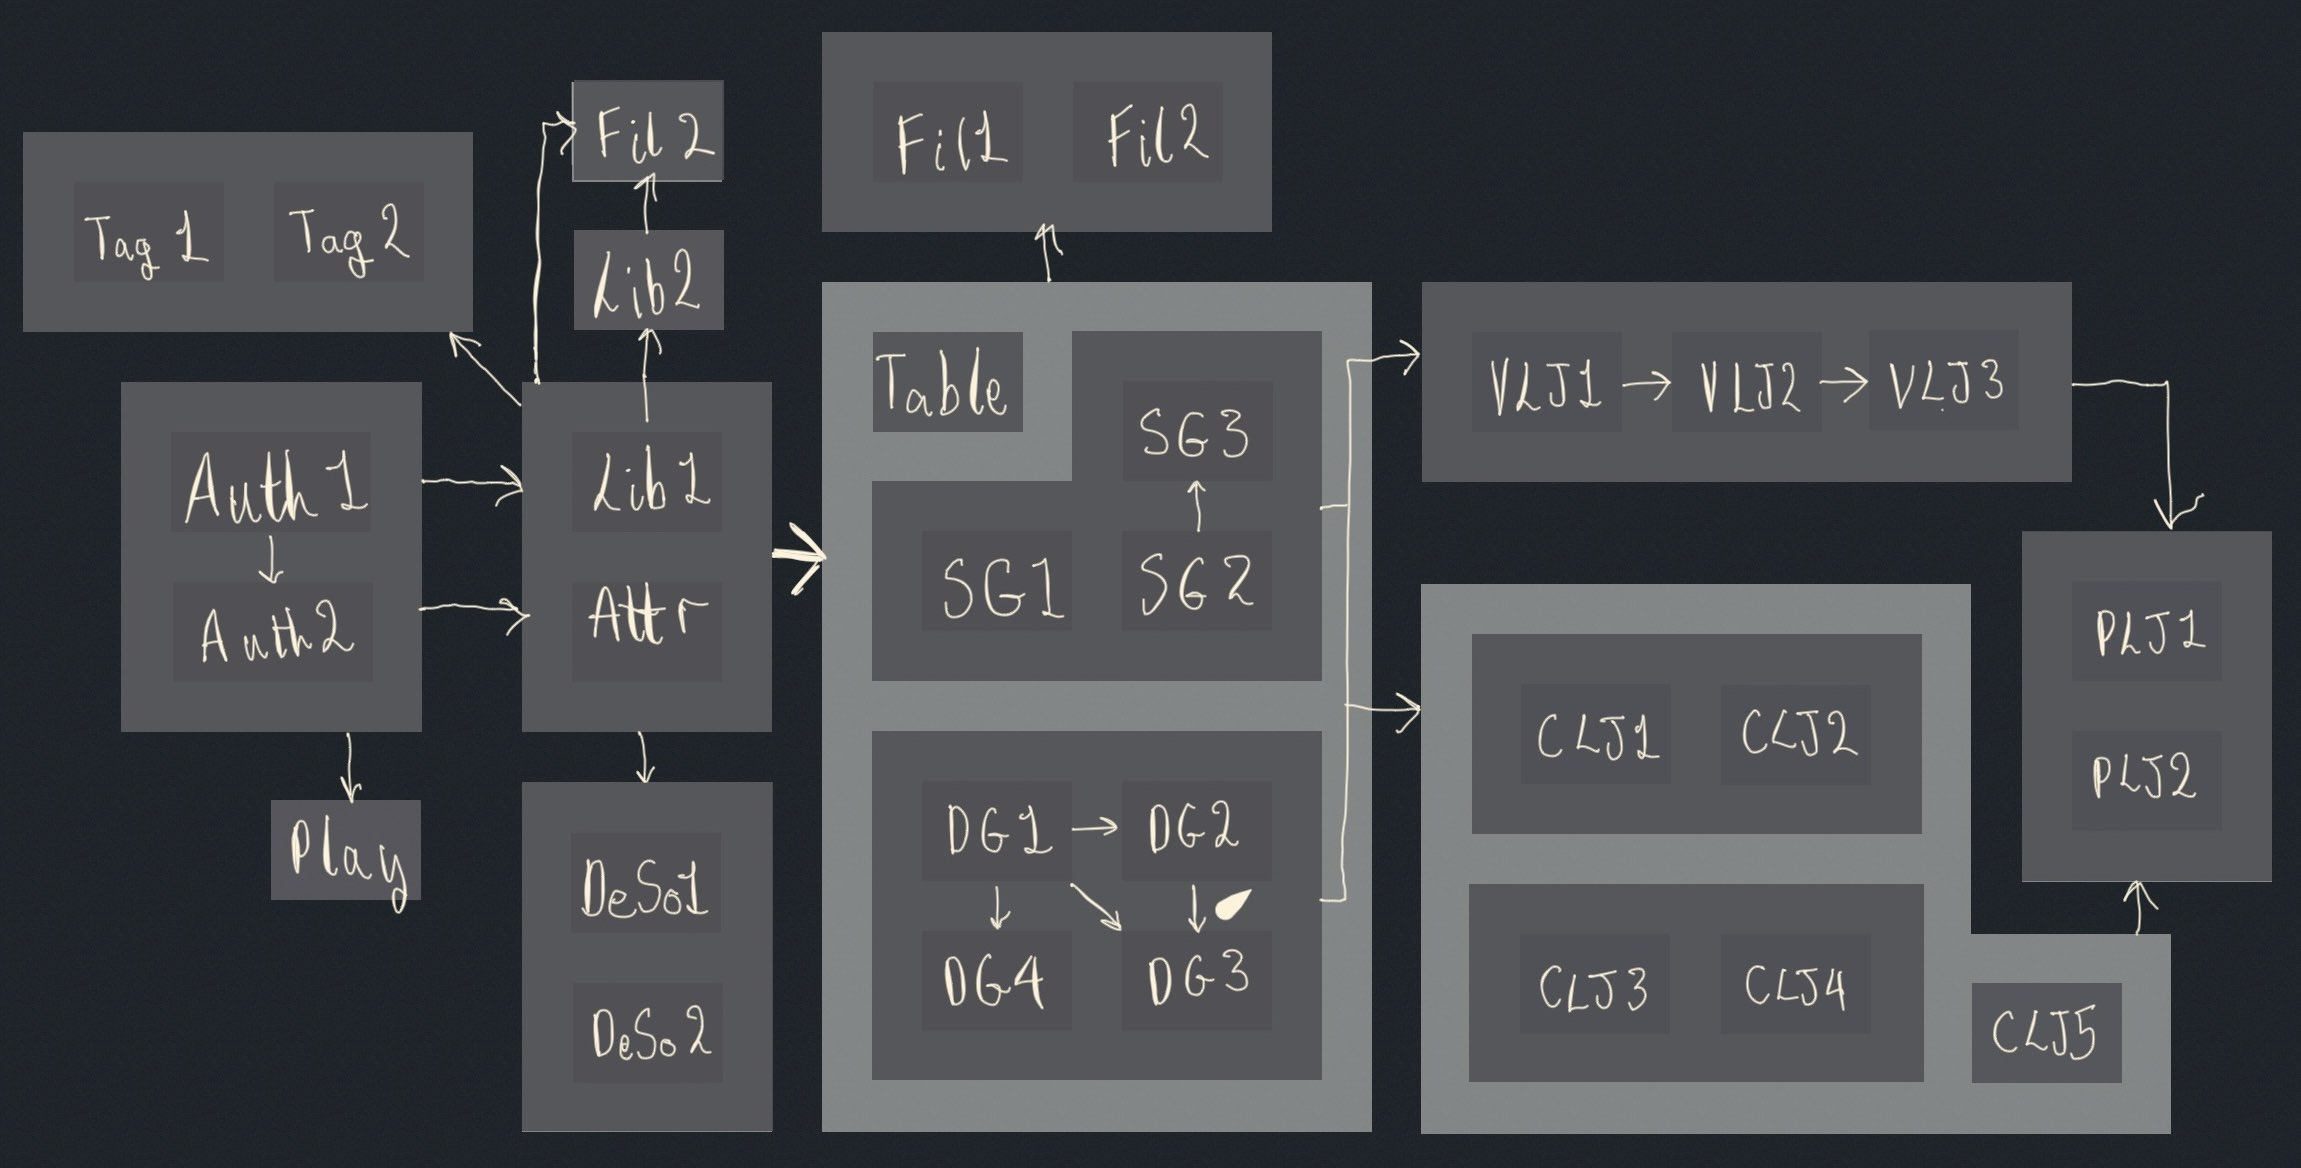
\includegraphics[scale=0.204]{Activity_Network_Diagram.jpg}
    \caption{Activity Network Diagram of Functional Dependencies}
\end{figure}

% User stories have been cut as it was deemed that their content overlapped too much with the functional requirements and as such were easy to cut to fit within the word limit

\section{TODO: Static Cartesian Graphs}
%* Explain how I coded this basically
[-] combine the different continuous attributes
[-] 

\section{Dynamic Similarity Graph}
[-] Each song is a node in the graph
[-] Each song has multiple bidirectional weighted edges to each other song
    [-] Discrete attributes/metadata: edge is overlap of discrete metric between song A and song B
    [-] Continuous attributes/metadata: weight of edge is the 1-x, where x is a the difference between the values of Song A's acousticness and Song B's acousticness (for example)
[-] When rendering the graph, songs are pulled closer together depending on strength of weight:
    [-] continuous weight of 100\% - songs pulled as close together as possible
[?] maybe have a toggle to turn off collisions? that way clusters that form might be more interesting or the graph never settles on a shape

\section{Audio Journeys}

\section{TODO: UI Wireframes}%* can categorise them by the feature roadmap? Or maybe I can group sections of the roadmap
As one of the key non-functional requirements is for the developed features to integrate into existing streaming applications, the UI was designed using Spotify's desktop interface as an inspiration.

\section{TODO: Storyboards}%? How many do I have of these?

%todo how do I fit this into the project. Is it design or development
%TC: ignore
\begin{longtable}[c]{|c|c|c|p{5em}|p{5.5em}|}
    \caption{The Echo Nest Attributes}\\%todo better caption
    \toprule
    \textbf{Attribute} & \textbf{Definition} & \textbf{Datatype} & \textbf{Possible Values} & \textbf{Continuous /Discrete} \\
    \midrule
    \endfirsthead

    \textbf{Acousticness} & & \texttt{float} & \texttt{0}-\texttt{1} & \multirow{9}{*}{Continuous}\\*
    \cmidrule{1-4}
    \textbf{Danceability} & & \texttt{float} & \texttt{0}-\texttt{1} & \\*\cmidrule{1-4}
    \textbf{Energy} & & \texttt{float} & \texttt{0}-\texttt{1} & \\*\cmidrule{1-4}
    \textbf{Instrumentalness} & & \texttt{float} & \texttt{0}-\texttt{1} & \\*\cmidrule{1-4}
    \textbf{Liveness} & & \texttt{float} & \texttt{0}-\texttt{1} & \\*\cmidrule{1-4}
    \textbf{Loudness} & & \texttt{float} & \texttt{-60}-\texttt{0} & \\*\cmidrule{1-4}
    \textbf{Speechiness} & & \texttt{float} & \texttt{0}-\texttt{1} & 
    \\*\cmidrule{1-4}
    \textbf{Valence} & & \texttt{float} & \texttt{0}-\texttt{1} & \\*\cmidrule{1-4}
    \textbf{Tempo} & & \texttt{float} & \(\ge\)\texttt{0} & \\*
    \midrule
    \textbf{Key} & & \texttt{integer} & \texttt{None}/\texttt{C}/\texttt{C\#} /\texttt{D}/\texttt{D\#}/\texttt{E}/\texttt{F} /\texttt{F\#}/\texttt{G}/\texttt{G\#}/ \texttt{A}/\texttt{A\#}/\texttt{B} & \multirow{3}{*}{Discrete}\\*
    \cmidrule{1-4}
    \textbf{Mode} & & \texttt{boolean} & \texttt{true}/\texttt{false} & \\*
    \cmidrule{1-4}
    \textbf{Time Signature} & & \texttt{integer} & \texttt{3}/\texttt{4}/\texttt{5}/\texttt{6}/\texttt{7} & \\*
    \midrule
    
\end{longtable}
%TC: endignore
%% Building off of the above what is the design of the
%% final approach that I went with

% -------------------------------------------------
% Development Process (%? do I talk about the project planning here?)
% -------------------------------------------------
%% ----------------------------------------------------------------
%%? 1st Draft In Progress
%% ---------------------------------------------------------------- 
\chapter{Development (1100 words)}
\section{Chosen Techonology Stack}
\subsection{Application Framework: Tauri vs Electron}
Tauri and Electron are the two main frameworks for building native applications using web technologies. They both create an executable than can be run on any operating system. Electron bundles a version of Chromium into the executable, increasing the size of the application compared to Tauri, but resulting in a consistent experience across any OS. Tauri uses the default browser of the operating system, which means it is smaller in size, but more inconsistent. As the application will mainly be tested using Windows machines, this inconsistency is not an issue.

The main difference between Tauri and Electron resides in the backend; Electron is JavaScript-based, whilst Tauri is Rust-based. Due to the type-safety and prior experience in Rust, Tauri is the more optimal choice for the backend. Tauri also integrates with any frontend framework much simpler than Electron does (Electron requires more manual setup). 

Tauri is less widely-used than Electron however, meaning there is less community support. However, Tauri is still well-documented and has very open forums for support.

As both frameworks use web technologies, accessing a user's music collection via API is trivial.

\subsection{Frontend Library}
React.js was chosen as the frontend framework for this project for the following reasons:\begin{itemize}
    \item[\textbf{+}] Breaks down the code into reusable components that can be inserted and removed easily.
    \item[\textbf{+}] Virtual DOM: only the parts of the UI that have changed are re-rendered, meaning the entire UI doesn't have to re-render for any update
    \item[\textbf{+}] Widespread adoption (highest community and industry use), lots of support and excellent documentation
    \item[\textbf{+}] Full compatibility with three.js, an excellent 3D data visualisation library.
    \item[\textbf{+}] Highly effective at managing state.
    %\item[\textbf{-}] Learning time required
\end{itemize}

\subsubsection{Data Visualisation}
Whilst using a specialised data visualisation library would be easier to use and intepret, it would be too restrictive in making the views interactive. As such three.js a 'lower-level' library was chosen even though it requires more work to create the static cartesian graphs.

Three.js was chosen partly due to its synergy with React (via the \lstinline|react-three-fiber| library) and mostly for its more flexible nature. This library allows the user to build complex 3D scenes using primitive 2D and 3D shapes. As such it works well for creating the static and dynamic graphs, polar charts and ridge plots.

\subsection{Backend}
\subsubsection{Database: Entity Component System}
To store a user's songs, collection structure and the song attributes a local storage approach was taken. Cloud-based would be effective at allowing for access from multiple devices, however this was considered out of scope and not worth the extra development.

To efficiently store and query the data locally, the \lstinline|flecs| library (which has Rust bindings) was chosen:\begin{itemize}
    \item[\textbf{+}] Entity Component System - alternative paradigm to object-oriented programming, execellent at storing and querying large amounts of data efficiently, very good at parallelising complex logic. Mainly used for game engines.
    \item[\textbf{+}] Rust-bindings and very lightweight \(\to\) slots easily into the project %with a minor bit of faff
    \item[\textbf{+}] Rich support for relationships \(\to\) easy to create and query graphs using the data.
\end{itemize}

This heavy support for relationships helps with storing and accessing the structure of a user's collection. It also makes it easy to create the dynamic graph view.

Bevy, another ECS library written in Rust was considered, however it has significantly worse support for relationships and is less featureful in general.

%%%* Should have just put the API keys and stuff in a singleton or something in the flecs world. Would've meant that I could use the API tokens without needing to pull it from state.

\section{Accessing a user's Digital Music Collection}
There are many applications that allow for streaming music and creating music collections. Most of these applications have an API to easily work with, however these vary in their effectiveness. The chosen streaming application for this project was Spotify:\begin{itemize}
    \item[\textbf{+}] Extensive and reliable API
    \item[\textbf{+}] Free API access (Premium account required for controlling playback and song queues)
    \item[\textbf{+/-}] endpoints for detailed attributes for any song (now deprecated)
    \item[\textbf{-}] Risk of API deprecation or major breaking changes to the API
\end{itemize}

Whilst there have been major changes to the API that significantly affected the project, this API is still the most feature complete and easiest to use.
%? maybe make the below a list to reduce word count/streamline this section
Apple Music was considered due to also having a considerable market share and extensive API, but was not chosen due to not wanting to be locked to iOS users. YouTube music, another popular streaming service, was considered however they have no official API.

Pandora is a US-based streaming service that also has attributes on their songs in their Music Genome project, however their API is paywalled and region locked to the USA. Amazon music also has a high market share but their API is only in a closed beta so it was not considered.

\section{Sourcing the Echo Nest Attributes}
Initially Spotify was the source for fetching song attributes as Spotify was already the chosen API for accessing a user's music collection.

However, due to Spotify's deprecation of these endpoints (\lstinline|Get Track's Audio Features| and \lstinline|Get Track's Audio Analysis|) an alternative method was required. For most of the development process SoundCharts's API was used. This was then switched to Exportify instead due to reasons explained in the project retrospective. Where relevant both workflows will be shown in this chapter.

Note that if the more ideal approach is using Exportify.

\subsection{SoundCharts}
SoundCharts has an API that allows for fetching songs with the Echo Nest attributes attached. However, these attribute values are to a significantly lesser precision. Another issue with the API is that it is paywalled. There is a free trial, however this was only for 500 API calls which was only sufficient for development and not the final evaluation.

\subsection{Exportify}
Exportify allows for the exporting of one's Spotify collection as csv files with all associated metada and attributes. These attributes are also the original precision of Spotify's endpoints.

A minor bug/issue with the Exportify process is that the explicit field was not correctly filled in, meaning that all values in the csv were left empty. How this affected the project is also detailed in the Project Retrospective chapter.

\section{TODO: Architecture}%! what do I put here???
Diagram of the way I used the tauri API to effectively just access the flecs backend. Although the way I sent data and received data was a bit clunky. Should I have made a trait that allowed things to work together well?

[-] someone interacts with the react frontend, ts function calls \texttt{invoke("rust\_function")} by using tauri API
[-] tauri finds the unique function with name \texttt{rust\_function} and runs that function
[-] if that function needs to access the songs/collection a flecs query is created and run.
[-] data is then sent back to the frontend via listening for events or as the callback to the frontend function that did the invoking

\section{TODO: Application State Flow}
Application state diagram

\section{TODO: Development Methodology}
[-] Decided on a agile customer driven approach.
[-] had a meeting with Dhruv + Josh who said that maybe think more about playlists so planned to start thinking about the project in terms of looking at specific playlists. Started off with library during development as that was easiest.
[-] did learn lots of things that would be cool but out of scope
    [-] the 3d static+dynamic graphs would be good for AR/VR
    [-] learnt that Dhruv is fully active and Josh is more passive wants to listen around a song
[-] was supposed to do another meeting on a mvp but didn't finish in time to organise meeting before the evaluation

\section{TODO: How I coded the features like the graphs}

%%% Talk about how I coded the project, being more pseudocodey, as in more alluding to how the code works, so it could be theoretically replicated in another language.
%% After I designed what I was making, how did I go
%% about implementing the actual project

% -------------------------------------------------
% Testing + Results
% -------------------------------------------------
%% ----------------------------------------------------------------
%%? 1st Draft Completed
%% ----------------------------------------------------------------
\chapter{Testing and Results (1800 Words)}
\section{Data Collection}
As the project was aiming to initially understand how people manage and use their digital music collections, then to see how these could be transformed using new concepts implemented with software, a more open approach was required.

Students from the University of Southampton with an active Spotify Account were invited to take part in a participant study after development had finished. This study was performed and complied with the ethics standards set out in \lstinline|ERGO78677.A2|.

The study consisted of 1-on-1 ethnographic semi-structured interviews, typically lasting 45-60 minutes. The process was as follows:\begin{itemize}
    \item Provide the participant with an information sheet and consent form
    \item They were then asked how they build song queues - from fully random to fully ordered
    \item The following questions were asked:\begin{itemize}
        \item How is your collection organised?
        \item How do you maintain your collection?
        \item How do you create queues to listen to? (expanding on their previous answer of random vs ordered)
        \item How do you interact with your listening queues after creation (excluding the listening aspect itself)?
    \end{itemize}
    \item Then the participant loaded a playlist into the software application:\begin{itemize}
        \item Export a chosen playlist as a \lstinline|.csv| file from the Exportify web page
        \item \item Open the Audyssey application with the aformentioned \lstinline|.csv| file
    \end{itemize}
    \item Then the user was walked through the application and then they gave their thoughts on the application and concepts within it.
\end{itemize}

Due to the semi-structured nature, some questions and topics were explored to different degrees depending on the different answers and behaviours of the participants. During the interviews, notes were taken to be used in an inductive coding process.

This process was done iteratively, modifying and combing codes after each interview. Then these codes were grouped to form a hierarchy of themes and sub-themes, along with the occurrence count for each code. This process follows from the Thematic Analysis process set out by \cite{
    %todo Joy, Braun, Clarke's paper on reflexive thematic analysis
}

%% ----------------------------------------------------------------
\section{(TODO Add quotes + who said what + fix longtable)Thematic Analysis of Interview Pre-application}
%TC: ignore
\begin{longtable}[c]{| c | c | c | c|}
    \caption{Hierarchical Table of Themes with Counts.} \\
    \toprule
    Theme & Sub-Theme & Code & Count\\
    \midrule
    \endfirsthead
    
    %\caption[]{Hierarchical Table of Themes, Sub-Themes, Codes and Counts.}
    \toprule
    Theme & Sub-Theme & Code & Count\\
    \midrule
    \endhead

    \multirow{9}{6em}{
        Collection Organisation
    } & \multirow{2}{*}{Method} & Singular Playlist & 2\\* \cmidrule{3-4}
            & & Multiple Playlists & 4 \\*
        \cmidrule{2-4}
        & \multirow{2}{*}{Full Collection Understanding} & Vague & 1\\*  
            \cmidrule{3-4}
            & & Strong & 5 \\*
        \cmidrule{2-4}
        & Mental Model & Distinctly Unique & 2 \\*
        & Familiar Structure & Easy to Use & 4 \\*% all the playlist peeps
        & Dark Spots & Forgotten/Unfamiliar Songs & 3\\*
        \cmidrule{2-4}
        & \multirow{2}{*}{Growing Song Count} & Always Adding & 6\\*
            \cmidrule{3-4}
            & & Doesn't Remove Songs & 5 \\*
    \midrule

    \multirow{5}{6em}{
        Playlist Management
    } & \multirow{5}{*}{Unique Identity} & Per Artist & 1 \\*
        \cmidrule{3-4}
            & & Per Time Period & 2 \\*
            \cmidrule{3-4}
            & & Per Genre & 2 \\*
            \cmidrule{3-4}
            & & Per Mood/Vibe & 3 \\*
            \cmidrule{3-4}
            & & Activity & 2 \\*
        \cmidrule{2-4}
        & \multirow{4}{*}{Friction/High Mental Load} & Creating DesiredPlaylists & 2\\*
        \cmidrule{3-4}
            & & Switching between Playlists & 2\\*%* for creating queues
            \cmidrule{3-4}
            & & Infrequent Playlist Creation & 3\\*
            \cmidrule{3-4}
            & & Cleaning Playlist Contents & 1\\*
        \cmidrule{2-4}
        & \multirow{2}{*}{Absolute/Fixed Ordering} & Playlist Contents &3\\*
        \cmidrule{3-4}
            & & Specific Audio Experiences & 3\\*
    \midrule
    
    \multirow{12}{6em}{Listening Journeys (Queue)} & \multirow{2}{*}{Creation Process} & Passive: Shuffle & 5\\*
    \cmidrule{3-4}
            & & Active: Manually Create Queue & 2\\*
        \cmidrule{2-4}
        & \multirow{3}{*}{Source} & Individual Playlist & 4\\*
        \cmidrule{3-4}
            & & Full Collection & 4\\*
            \cmidrule{3-4}
            & & Affected by Recency Bias & 3\\*
        \cmidrule{2-4}
        & \multirow{3}{*}{Shuffle} & Unplayed Songs & 2\\*
        \cmidrule{3-4}
            & & Fixing the Queue & 4\\*
            \cmidrule{3-4}
            & & Close Enough & 2\\*
        \cmidrule{2-4}
        & \multirow{2}{*}{New Song Buffer} & Forgetting to Add & 3\\*
        \cmidrule{3-4}
            & & Desired & 2\\*
        \cmidrule{2-4}
        & \multirow{2}{*}{Listening as a Trajectory} & Listening Rendered as a Line & 4\\*
        \cmidrule{3-4}
            & & Boundary Songs & 2\\*%* Which they change direction on
    \midrule
\end{longtable}
%TC: endignore

\subsection{Collection Organisation}%todo add Quotes
All the participants had a specific way that they digitally organised their Spotify music collections. Mainly they could be split into two groups: those who placed all their songs into one singular box (the Liked Songs folder) or those who split their collection over multiple playlists.

Only 1 participant felt like they had a vague understanding of their entire collection [Riya], whilst the other 5 felt like they had quite a good grasp on their collection.

Contradicting this however, 3 of the aforementioned 5, upon exploration of their collection in the software application realised there were forgotten or unfamiliar songs to them in their collection.
%? This implies that their grasp on their collection is not as concrete as they stated.

3 of the 4 participants who utilised multiple playlists to organise their collection also attributed benefits to this:\begin{itemize}
    \item knows where a song would be found in, doesn't have to know the exact location, taking off mental load
    \item muscle memory, familiarity
\end{itemize}
%* Implying that this organisation and seperation into distinct regions is good, but as we will find later this level of organisation requires a lot of effort and once it is lost is difficult to regain
The participant who didn't attribute benfits to the structure of their playlists also had an issue with their playlists converging to the same identity[Riya: "over time, my playlists all sort of converge to the same type of song, though they're not meant to"]

Common across all 6 participants is that their collections were continuously growing over time, with only 1 participant stating that they removed songs[Riya] although rarely. %? and only cuz they didn't really belong in the first place

\subsection{Playlist Management}
The 4 participants who organised their collection using playlists also had common concepts and behaviours.

All 4 participants created their playlists with a distinct identity in mind whether this be for a specific artist[Shruthi], a time period[Shruthi, Vedarth], a genre[Josh, Vedarth], a mood or vibe[Riya, Josh, Vedarth] or an activity like the gym[Vedarth, Casper wanted one].

Many of the participants however noted common cases where they felt friction in interacting with their playlists. 2 participants[Shruthi, Vedarth] felt that it was "too much effort" to create playlists with distinct identities that they felt were missing from their collection as there are "too many songs" and ["it would take too much time"].

%? do I need to move this to a different section?
2 participants also noted that when switching between playlists to create queues, they felt that there was a significant amount of mental effort required that put them off from doing so, even though they mentall felt that they needed to create the queue.

3 of the participants also mentioned that they make playlists very infrequently, with 2 of them only making them for each new time period. This was due to ""[insert quote about how much effort it was]

Something that didn't cause friction was the absolute or fixed ordering of the contents of their songs. 3 participants ordered by time[Vedarth, ] or alphabetical order[Shruthi], all remarking that this consistnent order provided "muscle memory" and aligns+reinforces with their mental model
%? Do I have the last bit here?
3 of the participants also ordered songs in the collection to elicit a specific listening experience. 1 participant[Casper] only listened to albums in their canonical order as they exclusively enjoyed that way of listening to them. The other two participants ordered them so that when the didn't shuffle, they could listen through that experience they set out for themselves.

\subsection{Listening Queues}
There were two modes of creating listening queues for the participants: 5 had a passive mode where they created their queues using the shuffle features and 2 created their queues by manually placing songs in the queue.

4 participants built these queues from an individual playlist[] and 4 built them from their entire collection[Casper, Roberto]. When choosing which playlist to choose from and what song to start listening to, 3 participants said that their choice was affected by a recency bias. They felt that they "had a good chance of forgetting songs that were added to the collection earlier on".

Passive listeners also had issues with the shuffle feature of randomly creating an order. 4 participants felt that they had to fix or guide the queue manually due to the shuffled order creating a listening experience that did not match their expected mental queue.

2 participants[] mentioned that they would keep skipping songs if it did not match their expectations until they reached one that was "close enough"[]. % Do I talk about how this is effort and annoying to do? Can't really because I didn't ask this although I should've, can at least bring it up in the project retrospective

2 participants[Josh, Riya] did state that even if the shuffled queue was giving a song that wasn't what they wanted, they would not change it partially due to "not being bothered" and if the playing song was "close enough" to what they were subconsciously expecting.

2 participants[] also mentioned that whilst they used the shuffle feature frequently, they felt/knew that there were songs that hadn't been played for quite some time as the shuffle simply wasn't playing them. This meant that they weren't fully experiencing their collection.

%todo This is sort of duplicated across the evaluation section as well
\subsubsection{New Song Buffer}
3 participants[] mentioned that when they listen to songs passively and are "less aware of what I'm listening to"[Casper?] that they can forget to add these new songs to their collection. 1 participant[Riya] also mentioned that after adding a new song to their collection they would sometimes remove it on subsequent listens due to realising they didn't actually like it. As such 2 participants[] mentioned that they would like a user-facing buffer region feature where newly listened to songs could be permanently added/removed after a few listens.% This would help with managing their collection

\subsubsection{Listening as a Trajectory}
%todo I can probably put in other stuff here to create a proper narrative flow or do I leave that for the final discussion evaluation part?
4 participants mentioned wording that indicated they understood their listening journey to have a direction which was sometimes reflected in the queue. 2 participants[Riya, Josh] mentioned that a factor deciding how they actively mentally change listening direction is when they are on a boundary region of their collection. "When I listen to this song, it has a sad part that'll make me want to listen to more sad songs instead of the direction the queue is currently heading in".

%% ----------------------------------------------------------------
\section{Application Feedback}
Before, the interviews were aimed at undrestanding how the participants organised their digital music collection and how they build and listen to queues using this collection. Whilst using the applicatio, the interview changed to being more about gaining feedback on the usability of the system and each individual feature implemented. Any features that the participants felt would be useful (after interacting with the application) were explored in detail.

As the participants interacted with the application they were asked for their feedback on the implemented features and the attributes:
%todo add in table but what headings?
%todo Attributes/Metadata
%todo Graph feedback
%% ----------------------------------------------------------------
\subsection{Feedback: Attributes/Metadata}

%% ----------------------------------------------------------------
\subsubsection{Value Accuracy}
2 participants disagreed with some of the attribute values for songs in their collection, noting that it did not align with what they expected.
%! However, a lot of people were also like they agreed with it though

%% ----------------------------------------------------------------
\subsubsection{Attribute Opinions}
%% ----------------------------------------------------------------
\paragraph{Key, Mode, Time Signature}%todo
Some cared, some didn't care.

Overall these are more useful in the calculating similarity and also being able to be toggled off (although the toggle off is probably unnecessary as no-one said they actively didn't want it there)

%% ----------------------------------------------------------------
\paragraph{Attribute Rankings: Time above all else}%todo REWORD
[Vedarth] noted that the time axis was easier to understand and more interested in as time/history is more familiar to them. [Casper] also noted that a sped up line of their audio history would be cool, also implying that time was a instinctively useful attribute

\paragraph{Attribute Combinations: Overwhelmed with Choice}%todo REWORD
Many participants[] noted that though specific combinations were interesting they were overwhelemed with trying to find specific combinations and weren't sure where to start or what to do.
X participants agreed that they would like \textbf{customisable presets}, where they could be given combinations to look at that provide easily digestible insights. Using these combinations as a base, the users' could then explore to find their own preferred combinations.

\paragraph{Distributions: Liked seeing ways of representing their Music Taste}%TODO

\paragraph{Desired Feature: Ridge Plot of Histograms for Individual Histograms}%TODO

\paragraph{Attribute: Extreme Ends}%todo FIX
Liked seeing the extreme ends for each attribute (i.e. top 5) although this could be due to the fact that the table view made it easy to see this.
1 participant[Casper] noted that these extreme ends would be useful for automatically creating high danceability playlists for example. There is alreay projects that can do this, though it does beg the question, if we start combing attributes, what sort of playlists would be created. %* However this is something that would of only really been able to check by using the dynamic graph and being able to toggle which attributes are affecting the graph.

%% ----------------------------------------------------------------
\subsection{Feedback: Graph Model}
TODO NEXT

\subsubsection{Graph-Based Suggestions}
3 participants[] noted that they would appreciate seeing song suggestions that clearly show how they slot into their entire collection. Both the ridge plot and dynamic graph would be good for this as they both show the user's entire collection.

\subsubsection{}{Graph Navigation Controls}
Participants noted that the controls were good for navigating in the 2D graph. However, some particiapants[] felt that they would also like a 1st person style of controls, where they could fly through the space of songs. something akin to Minecraft's Creative Mode Controls
%todo maybe put an image of what keys correspond to what for this new controls system

\subsubsection{Song Identification}
Due to time constraints, setting the colour of a song sphere was unfinished. To understand what would be the most preferable dimension to distinguish songs, participants were asked during the study, with the below responses:\begin{itemize}
    \item by colour of\begin{itemize}
        \item Artist = 1[]
        \item Genre = 4[]
        \item Mood/Vibe = 3[]
        \item Discrete Metrics = 0, as participants felt that they would need to see it implemented to see if it would be useful
    \end{itemize}
    \item the image of the album the track belongs to (but only if there was enough visual space to render it)
\end{itemize}

\subsubsection{Dynamic Graph}
All 6 participants[] noted that they would've liked to see their collection using the dynamic graph feature.

All 4 of the participants[] who organised their collection using playlists also expressed interest in seeing how the potential clusters formed in the dynamic graph would map to their created playlists.

\paragraph{Songs as Listening Focus Points}
2 participants[] also noted that when they're listening they would like to be able to select songs as points to listen around (for queue generation and modification)
%% How did I test the application, both software + novel concepts

% -------------------------------------------------
% Evaluation of Results
% -------------------------------------------------
%% ----------------------------------------------------------------
%%? 1st Draft In Progress
%% ---------------------------------------------------------------- 
\chapter{Evaluation (1700 words)}
This project aimed to ask two research questions:\begin{itemize}
    \item \textit{how can the organisation of digital music collections be improved to better reflect people's mental models of their collections, without increasing the mental load required?}
    \item \textit{How can we improve the process of creating and controlling}
\end{itemize}

People have a expected mental audio journey. Passive listeners usually have much larger audio journeys that they'd be happy with

%% ---------------------------------------------------------------- 
% Active is blue, Passive is yellow (I don't know why)
\section{Active vs Passive Listening Spectrum}
%% ---------------------------------------------------------------- 
When someone is listening to a sequence of songs they exist somewhere on the passive-active spectrum. This spectrum is concerned with the number of possible song sequences that the person is satisfied listening to.

At the extreme end, a fully passive listener is satisfied with any sequence of any songs, no matter how similar or dissimilar the songs in the listening journey are.

At the other extreme end is a fully active listener, someone who has an exact set of songs that they want to listen to, in an exact order. This order may be for many reasons.

All the participants were somewhere on this spectrum when they were listening to their collection, some would stay in one place or would move about on the spectrum.
[-] Casper usually passive, but then switches to active to make sure that they listen to album in the correct original order
[-] Vedarth passive when doing more mindless activities, but when more focused, preferred to actively create the queue.

%todo draw this spectrum
The interactions made by users (regarding song queues) can be mapped to relative positions on this spectrum:
[-] 100\% Active -> Manually find song then click add to queue
[-] -> Shuffle a small playlist / Song radio
[-] -> Shuffle a large playlist

Keeping track of the next ~10 upcoming songs -> slightly active
Reorder queue -> active
Switch to new playlists -> temporary active then back to passive

\subsection{What is a Listening Journey?}
%% ---------------------------------------------------------------- 
%%* Listening Journeys
%% ---------------------------------------------------------------- 
A listening journey is simply a sequence of songs and as with any sequence, it has the following properties:\begin{itemize}
    \item Initial Item (First Song)
    \item Previous Item (Previously Played Song)
    \item Current Item (Currently Playing Song)
    \item Subsequent item (Next Song)
    \item End Point (Last Song)
    \item Length (Number of Songs Listened to)
\end{itemize}

However this sequence is not simply a sequence of scalar items, but should be thought of as a sequence of vectors, items with direction. As such the overall song queue can be thought of being a listening journey, with an overall direction (and a direction from song to song).

This direction is a vector in an n-dimensional space, where n is the total attributes and metadata for a song. This project only looks at a subset of these attributes and metadata -> the Echo Nest attributes and the Spotify metadata.

What we propose is that the full listening history of a user is comprised of these listening journeys.
However, due to the continuous nature of listening to music in the digital era, further research will have to be done to see if people still have 'end points' or final songs as this was not investigated during the participant study.

A listening journey has 3 parts: its history, its current position, its future:\begin{itemize}
    \item \textbf{History:} a list of songs ordered by when they were listened to (with how much of each song was listened to)
    \item \textbf{Current Position:} the current position in the currently playing track
    \item \textbf{Future:} the trajectory that the listener will follow, comprised of segments that either have a fixed or unfixed/random order:\begin{itemize}
        \item \textbf{Fixed} similar to the history this is a collection of songs which are played through in order
        \item \textbf{Unfixed} the next song to be played is randomly chosen from a collection of 1 or more songs
        \item \textbf{Trajectory} this is the n-dimensional vector between the next song and the current song
    \end{itemize}
\end{itemize}

Both viewing history and the currently playing track are easily viewable and interactable in Spotify (and other streaming services). Spotify does allow for creating and interacting with the future aspect of queues, both fixed and unfixed, however the process to do so still has some friction and can only be done over the entire queue:\begin{itemize}
    \item Fixed Order Queue \(\to\) the user must manually locate and add songs one by one to create a fixed order queue% simple process but can be tedious having to locate each song, especially if they are not stored together -> Vedarth + Riya
    \item Fixed Order Segment \(\to\) a user can reorder songs in the queue to ensure that those songs are played in a fixed order% very easy to do
    \item Unfixed Order Queue \(\to\) a user can click shuffle play to create a new queue of all the songs in a playlist, which have been shuffled to be in a random order. Also they can shuffle the queue once it exists to randomise the order of songs within it. % also very easy
    \item Unfixed Order Segment \(\to\) should a user want to listen to 5 songs in a specific order, then listen to 15 different songs in a random order, then another five songs in a fixed order, there is no built-in way to do this.\begin{itemize}
        \item First the user would have to wait until they've listened through the first 5 fixed order songs.
        \item Then they would have to remember the 5 fixed-order songs they want to listen to at the end and remove those songs from the queue
        \item They could then shuffle the remaining 15 songs to achieve an unfixed/random order.
        \item If they are happy with the shuffle then they can re-add the final 5 fixed-order songs.
        \item However, if at any point they want to reshuffle the queue (but only the random-order songs) they have to go through the entire process again.
    \end{itemize}
\end{itemize}

As can be seen above, whilst Spotify does allow for creating both fixed and unfixed queues, they do not have a way of easily creating unfixed sections of the queue (without losing any desired fixed sections). This project aimed to provide a way for accomplishing this by using the graph visualisations as a base.

Unfortunately, as explained in the Project Retrospective chapter, this feature was not implemented and as such could not be fully tested. However, many participants noted that they would like to see this feature added to Spotify so that they could create song queues with both fixed-order and unfixed-order sections in their queue.
%!-- Now what?? Should this have been in the introduction?

\subsubsection{Listening Journey Trajectory}
A listening journey can also be thought of in terms of its trajectory, both between 2 songs, and over multiple songs. These trajectories are comprised of n-dimensional vectors, where n is the sum of all attributes and metadata on a song.

This project aimed at visualising these trajectories by rendering the listening history and upcoming queue as a line in the dynamic graph view, thereby representing all the dimensions of the songs.

Unfortunately, this feature was not completed (as explained in the Project Retrospective Chapter) but when asked to the participants, they all expressed interest in seeing their past and future listening rendered as a directional line. As such this is a concept worth researching further into, to determine how useful it can be, as this was not able to be fully tested during this project.

\subsection{Song Sources for Building Queues}%TODO
When passively listening, listeners often have very little mental energy they want to allocate to controlling the music they listen to[Shruthi Quote]. The easiest way to do this is to pick a playlist and start listening within it.

As such, playlists are an effective solution at reproducing listening queues. For some, one large playlist is enough (often Spotify's Liked Songs) as the listener is happy to listen to any possible sequence of songs in that large playlist. However, for others, they do not want to listen to all their songs at once[Vedarth: larger playlists lose their shuffleability], so they decompose their collection into multiple distinct playlists.

These playlists contain songs which all have a common aspect, which forms the identity of the playlist. This can be anything from having a specific artist or genre in common, as well as being for a specific activity like a workout.

However, due to the enclosed nature of the playlists it is difficult to know how much they overlap and what the true full collection looks like unless they are combined and rendered as one.

Unfortunately, combining multiple playlists into one was a feature that was not implemented, but is worth investigating further. Many participants noted that they wanted to see how similar their playlists were to each other. Further research will be needed to analyse the behaviour of choosing what songs go into which song queues[Vedarth agreed with this]. This will be detailed further in the Future Work Section.

%% --------------
%% Difficulty in maintaining Playlists
%% --------------
\subsubsection{Difficulties in Maintaining Playlists}
%todo fix this paragraph
At first glance, these playlists seem like the perfect solution for easily recreating queues. However, maintaining these playlists can be difficult for some[Riya: playlists started to converge] and applying clean-up is usually avoided [Riya: can't be bothered to go through and remove songs] as listeners just want to listen to their music usually. They are not usually in the mood to perform spring cleaning on their collection.

There is also a perceived heavy mental load associated with the process of creating playlists and adding songs to them. [Vedarth: likes the design and identity of a playlist and pulling different songs together] This puts off user's from creating new playlists with new identities with songs from their collection.[Shruthi+Vedarth would like maybe 2010's playlists but cba to make it]

There is currently too much friction associated with creating playlists, even though there is a desire.

%todo find source to cite how iTunes song tags are good.
\paragraph{Automatic Generation of Playlists}
One possible solution that was proposed in this project, but not attempted due to being low priority was song tags. These are words or phrases that can be attached to any song (similar to the genre metadata) and were a core feature of Apple's iTunes. These song tags can then be used to automatically generate playlists for that tag, taking away the tedious labour from a user. This will be explained futher in the Future Work Section.

\paragraph{Buffer Zone}
Another issue with utilising playlists effectively is adding the right songs when they're found by the user and removing ones that don't belong anymore. Most of the participants didn't remove songs, but that was also because they were more certain that a song belong to the playlist. For the participant who was less certain if a song belonged then they would add it and remove it afterwards if they deemed it necessary. A few participants also noted that they didn't always remember to add songs that they liked listening to, so they would prefer to 

\section{Visualising using Continuous Attributes}
From the feedback gained after the users interacted with the software application (the Audyssey) the following table can be constructed:


\begin{longtable}[c]{| c | c | c | c | c|}
    \caption{Optimal views for 1 or more songs and 1 or more continuous attributes} \\
    \toprule
    & \textbf{Singular Song}
    & \textbf{Each Song} % in a playlist/ for a high number of songs
    & \textbf{Song Distribution}
    & \textbf{Extremities} %Both min and max
    \\
    \midrule
    \endhead

    \textbf{1 Attribute} & \multirow{3}{*}{Table} & Table/1D Graph & Histogram & Table \\*
    \cmidrule{1-1}\cmidrule{3-5}
    \textbf{2 Attributes} & & 2D Static Graph & \multirow{4}{*}{Ridge Plot} & 2D Static Graph \\*
    \cmidrule{1-1}\cmidrule{3-3}\cmidrule{5-5}
    \textbf{3 Attributes} & & 3D Static Graph & & 3D Static Graph \\*
    \cmidrule{1-3}\cmidrule{5-5}
    \multirow{2}{*}{\textbf{\>3 Attributes}} & Polar Chart/Table/ & \multirow{2}{*}{Dynamic Graph} & & Table/\\*
    & Line over Ridge Plot & & & Dynamic Graph \\*
    \midrule
\end{longtable}

The Static Graph view is optimal for seeing the values of each song for 2 and 3 attributes as it allows a user to explore their collection

% -------------------------------------------------
% Project Retrospective
% -------------------------------------------------
%% ----------------------------------------------------------------
%%? 2nd Draft Complete | TODO Missing Gantt Charts
%% ----------------------------------------------------------------
\chapter{Project Retrospective (1350 words)}
This chapter will go over the significant limitations and an improved ideal project plan.

%% ----------------------------------------------------------------
\section{Handling Complexity: Miro Mindmap}
%% ----------------------------------------------------------------
One of the major elements that significantly helped with planning the project and managing the complexity of the project was building a hierarchical mindmap in Miro (a highly flexible diagramming tool). The reason Miro's mindmap was useful was that it allowed for children nodes to be toggled, meaning that they were visually hidden, but still accessible.

This feature significantly helped in breaking down the mammoth complexity of the entire project. The project was decomposed into the high-level parts, getting more specific as the tree became deeper. These high-level parts can be seen in figure \ref{figure::miro::mindmap_high_level}. Expanded sections of this diagram can be found in appendix \ref{appendix::Miro}.
\begin{figure}
    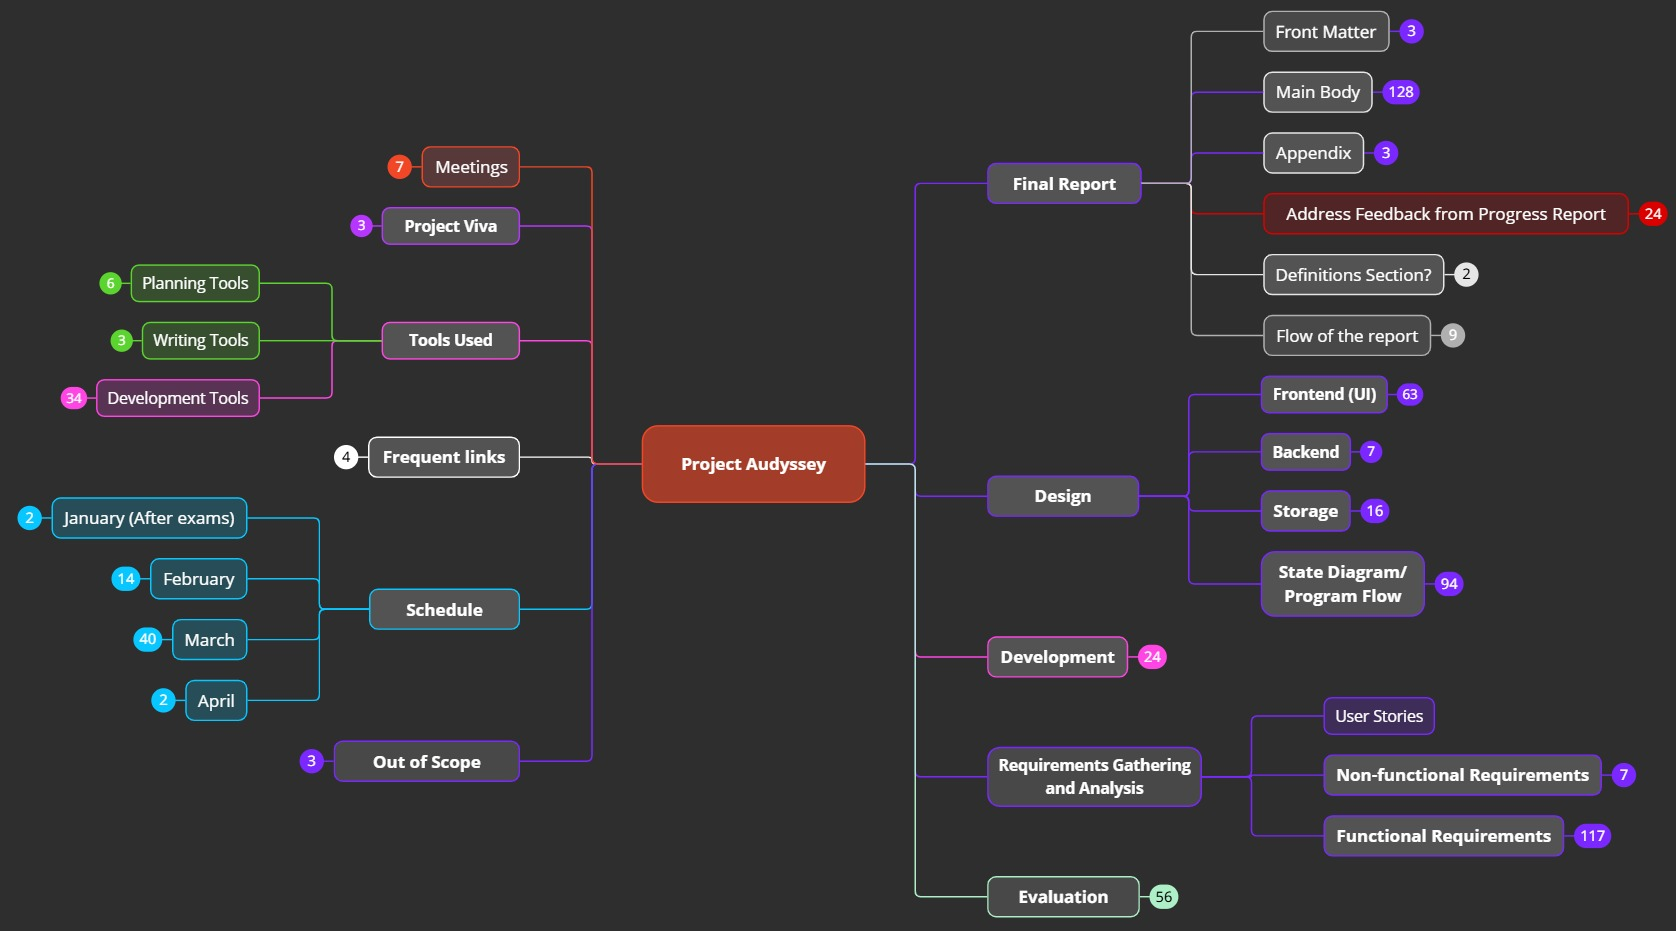
\includegraphics[angle=90, scale=0.43]{Miro_Mindmap_Depth_1,2}
    \caption{Miro Mindmap high level overview}
    \label{figure::miro::mindmap_high_level}
\end{figure}

The only issue with this diagram is the point at which it was used. This diagram was only built at the end of January meaning it was not helpful for the research and design stages, where it would have helped significantly.

%todo Do I add this because it doesn't reflect that well on me :(
The only drawback with this method is that whilst being able to hide child nodes is very useful, the count of hidden nodes is not that useful a metric. As such it was possible to hide nodes and forget about the contents which slightly hindered development.

%% ----------------------------------------------------------------
\section{Limitations}
%% ----------------------------------------------------------------
\subsection{Unfinished Code}
One of the key limitations of this project resides in the fact that the dynamic graph and audio journey features were not developed in time. This meant that these features were not able to be fully evaluated and therefore will require further research to truly understand them.

This is partly due to the unnecessary complexity in obtaining the Echo Nest attributes. The initial process to gain these attributes was through these endpoints via Spotify's API: \texttt{Get Track's Audio Features} and \texttt{Get Track's Audio Analysis}. However, as stated in \href{https://developer.spotify.com/blog/2024-11-27-changes-to-the-web-api}{this blog post}, these endpoints were deprecated.

As an alternative, I switched to using SoundCharts API to access the attributes. However, this API is paywalled and less precise but would still provide sufficient values for the graph views. Another issue with this workflow is that the complexity used up a lot of valuable development time. Had Exportify been found earlier, the project development phase would've been significantly smoother.

\subsubsection{Missed Opportunity to Reprioritise}
Whilst the SoundCharts workflow was unnecessarily complex, the other big issue is that the requirements should've been reprioritised. Whilst the static graphs provided a lot of insights as detailed in the evaluation, they were not the core focus of this project. Due to its novel nature, the dynamic graphs were more important and should've been re-prioritised once I realised that I would not have enough time to complete both graph views to a satisfactory standard.

The true/original niche/gap in the research was investigating better ways to create listening journeys, mainly using the graph visualisations as a foundation for controlling and viewing them. This is because, with the advent of the digital streaming era, there has not been any research for creating better tools for users. As discussed in the Evaluation, there is an expressed desire for these tools.

However, during development, after the static graph views were created, I realised that these were only really specifically useful in a data analysis perspective (something that has already been researched extensively (as mentioned in the Background chapter) and is not the focus of this project). The evaluation also confirmed this, as the participants felt that the static/cartesian graphs were only useful as a one-off and not as a basis for reflecting their mental model of their music collection.

In hindsight, developing the staic graph views should've been allocated to be done after the dynamic views so that the listening journeys could be accomplished as fast as possible. Static cartesian graphs were intially planned first as I did not realise at the time that they were significantly less useful for interacting with listening journeys than the dynamic view.

One participant in the evaluatory study also mentioned that they liked there being an absolute order to their songs/collection that they could return to. This absolute order synergises better with the dynamic graph, as the static graph produced different distributions for each combination of attributes on the axes.
%This was Vedarth, was there anyone else?

\subsubsection{Prototype Review Meeting Not Held}
A side-effect of the unfinished codebase is that there was not enough time to review the application before the evaluation. Whilst unfortunate this did not hold the project back too much as the software-related feedback was still obtained during the participant study (such as how to make the songs in the graphs easier to identify). However, more critical feedback would be ascertainable had the review meeting occurred.

\subsection{Evaluation: Small Participant Count}
Only 6 out of 10 participants were able to be evaluated in the participant study. Whilst these participants were varied in their listening and organisational styles and were sufficient for the evaluation, more would've been better to ensure the thematic analysis performed was as extensive as possible.

\subsection{Evaluation: Lengthy Interviews} %? (did I overscope?)
Another drawback of the evaluation interviews is that they were very lengthy, taking ~1hr on average. Whilst this in of itself is not an issue, considering two of the big features were not fully developed, the intended interviews would be even longer. As such, the interview should've been broken down into two parts:\begin{itemize}
    \item Understanding Participants' Music Organisation and Listening Style/Behaviours
    \item How the Audyssey affected their Music Organisation and Listening Behaviours
\end{itemize}
This first stage should've been done either before or after the design stage as it would also help inform the functional requirements for the system.

\subsection{Difficulties in Sourcing the Echo Nest Attributes}
As explained in the Background Chapter, the Echo Nest is a compnay that created a database of rich attribute data gained from high-quality analysis of song audio files. However, gaining access to these attributes has become increasingly difficult over the years:

\subsubsection{2014: Spotify buys EchoNest} EchoNest's extensive and free API is now locked behind a Spotify Premium Account. Whilst not a good event for the widespread community, this was not an issue for the project as the Spotify API was already a planned part of the project.

\subsubsection{Spotify Deprecates Key Endpoints}
\paragraph{27 Nov 2024} Spotify announces they are deprecating several endpoints for applications made after the 27th November - these endpoints included both \texttt{Get Track's Audio Features} and \texttt{Get Track's Audio Analysis} which were key for the project.

These audio features (or attributes) were critical for the project as they were the basis for graphing the songs and helping control the audio journeys.

To ensure that this didn't derail the project, an alternative was quickly found: the SoundCharts API. This API had an endpoint, that given a track's Spotify ID, would provide the attribute data that Spotify had deprecated access to.

However, this data was less accurate (only to 2 decimal places) and was also behind a paywall. For one month, the cost of access for 500,000 API calls at a 30\% academic discount amounted to 125 USD. This was within the budget of the project. Initially, the plan was to purchase one month once development had finished. As such the API access would be used only when it was fully needed.

\paragraph{Late March 2025} Due to significant issues with purchasing the API access using the University's system, another alternative method to gaining the attributes had to be found. This solution was found in Exportify, a web tool built by Pavel Komarov. This tool accesses the Spotify API, including the newly deprecated endpoints, to allow for exporting a spotify user's library to a \lstinline|.csv| file.

This tool was made before the deprecation announcement and is free to use, making it a very suitable replacement. Futhermore, the attribute values are to the original precision as provided by Spotify. The tool also allowed for exporting of individual playlists, making it easier for my software application to know how one's full collection was composed by the playlists and the catch-all liked songs.

\subsection{Scope Creep: Implementing Better Listening}
The goals for this project can be separated into two unique (but heavily linked) parts: improving large-scale music organisation and improving ways to control listening to music libraries.

As can be seen in the project brief the better listening was the initial focus, but during the research stage this pivoted to improving the organisation of large music libraries. When this pivot was made, improving better listening should've been re-classified as out of scope to ensure the project expectations remained manageable within the allotted timeframe.

However, improving better listening is a core aspect that affects how people organise their music libraries as found in the evaluation.

%% ----------------------------------------------------------------
\section{TODO: Initial vs Final vs Ideal Project Plan}
%%? how much explanation do I need, will Gantt charts be enough
%% ----------------------------------------------------------------
Below are three project plans:\begin{itemize}
    \item \textbf{Initial Plan} \(\to\) the planned progress of the project (created before the development stage)
    \item \textbf{Actual Progress}
    \item \textbf{Ideal Plan} \(\to\) upon retrospection, this is how the project should be approached if to be done again
\end{itemize}

%% ----------------------------------------------------------------
\subsection{Initial Plan}%todo Gantt Chart
%% ----------------------------------------------------------------

%% ----------------------------------------------------------------
\subsection{Actual Progress}%todo Gantt Chart
%% ----------------------------------------------------------------

%% ----------------------------------------------------------------
\subsection{Ideal Plan}%todo Gantt Chart
%% ----------------------------------------------------------------

%% From a planning perspective
    %% what went well? :)
    %% what went wrong? many, many things :(

% -------------------------------------------------
% Conclusion + Future Work
% -------------------------------------------------
%% ----------------------------------------------------------------
%%! Not Started
%% ---------------------------------------------------------------- 
\chapter{Conclusions}% Treat this as a continuation of the introduction, sumarising all the prior sections.

%* This is under the Lessons Learned heading in Notion

\section{Future Work}
[-] Auto-generating Playlists, possibly using song tags as a base
[-] Buffer zone for songs that have been rrecently listened to
    [-] added/viewable in collection but show that they aren't fully part of the collection yet
    [-] if this grows too much might come across the issue of people not wanting to deal with it.
    [-] need to be careful to figure out how to make it actually useful and not overwhelming for a user
    [-] how does this relate to song suggestions? are they one and the same or close enough??
[-] Rendering listening history

% \backmatter means that we've gone from 1,2,3,4,5 chapter numbering
% to unnumbered bibliography/appendices.
\backmatter

% -------------------------------------------------
% References
% -------------------------------------------------
\bibliographystyle{src/IEEEtran}
\bibliography{master}

% -------------------------------------------------
% Appendices
% -------------------------------------------------
\appendix
%% ----------------------------------------------------------------
%% Appendix.tex
%% ---------------------------------------------------------------- 
\chapter{Appendix A: Photos} \label{appendix1}
This is an appendix

\chapter{Appendix B: Code Listings} \label{appendix2}
This is an appendix
% Risk Assessment (maybe updated)
% More Detail on Miro Diagram?
% Project Brief

\end{document}

%%% Local Variables:
%%% mode: latex
%%% TeX-master: t
%%% End: